%%%%%%%%%%%%%%%%%%%%%%%%%%%%%%%%%%%%%%%%%%%%%%%%%%%%%%%%%%%%%%%%%%%%%%%%%%%%%%%%%%%
%%%%%%%%%%%%%%%%%%%%%%%%%%%%%%%%%%%%%%%%%%%%%%%%%%%%%%%%%%%%%%%%%%%%%%%%%%%%%%%%%%%%
%%
%%   Test Plotting
%% 
%%%%%%%%%%%%%%%%%%%%%%%%%%%%%%%%%%%%%%%%%%%%%%%%%%%%%%%%%%%%%%%%%%%%%%%%%%%%%%%%%%%%
%%%%%%%%%%%%%%%%%%%%%%%%%%%%%%%%%%%%%%%%%%%%%%%%%%%%%%%%%%%%%%%%%%%%%%%%%%%%%%%%%%%%

\documentclass[onecolumn]{emulateapj}
%\linespread{2.6}
\usepackage{graphicx, subfigure}
\usepackage{amsmath, natbib, listings}
\usepackage[bottom, hang, flushmargin]{footmisc}
\usepackage[urlcolor=magenta,citecolor=green,linkcolor=red]{hyperref}
\usepackage{appendix}
\usepackage{rotate}
\usepackage{adjustbox}
\usepackage{placeins}



\begin{document}
	

	\title{Python Group Plotting Test}
	
	\author{
		John D. Timlin}
	
	\date{\today}
	
	%\begin{abstract}
	%	We measure the two-point autocorrelation function of photometrically determined quasar candidates from the \emph{Spitzer} IRAC Equatorial Survey (SpIES) in the redshift range $2.9 \le \mathrm{z}\le 6$.
	%\end{abstract}
	
	\clearpage
	
	\section{Testing}
	
	Here is an example of what the new plotting parameters output. The figure on the left uses most of the default python plotting parameters, the only changes that were made was increasing the linewidths of the axes and lines in plot, and changing the font from sans-serif to serif.
	

	
	\begin{figure}[!h]
		\centering
		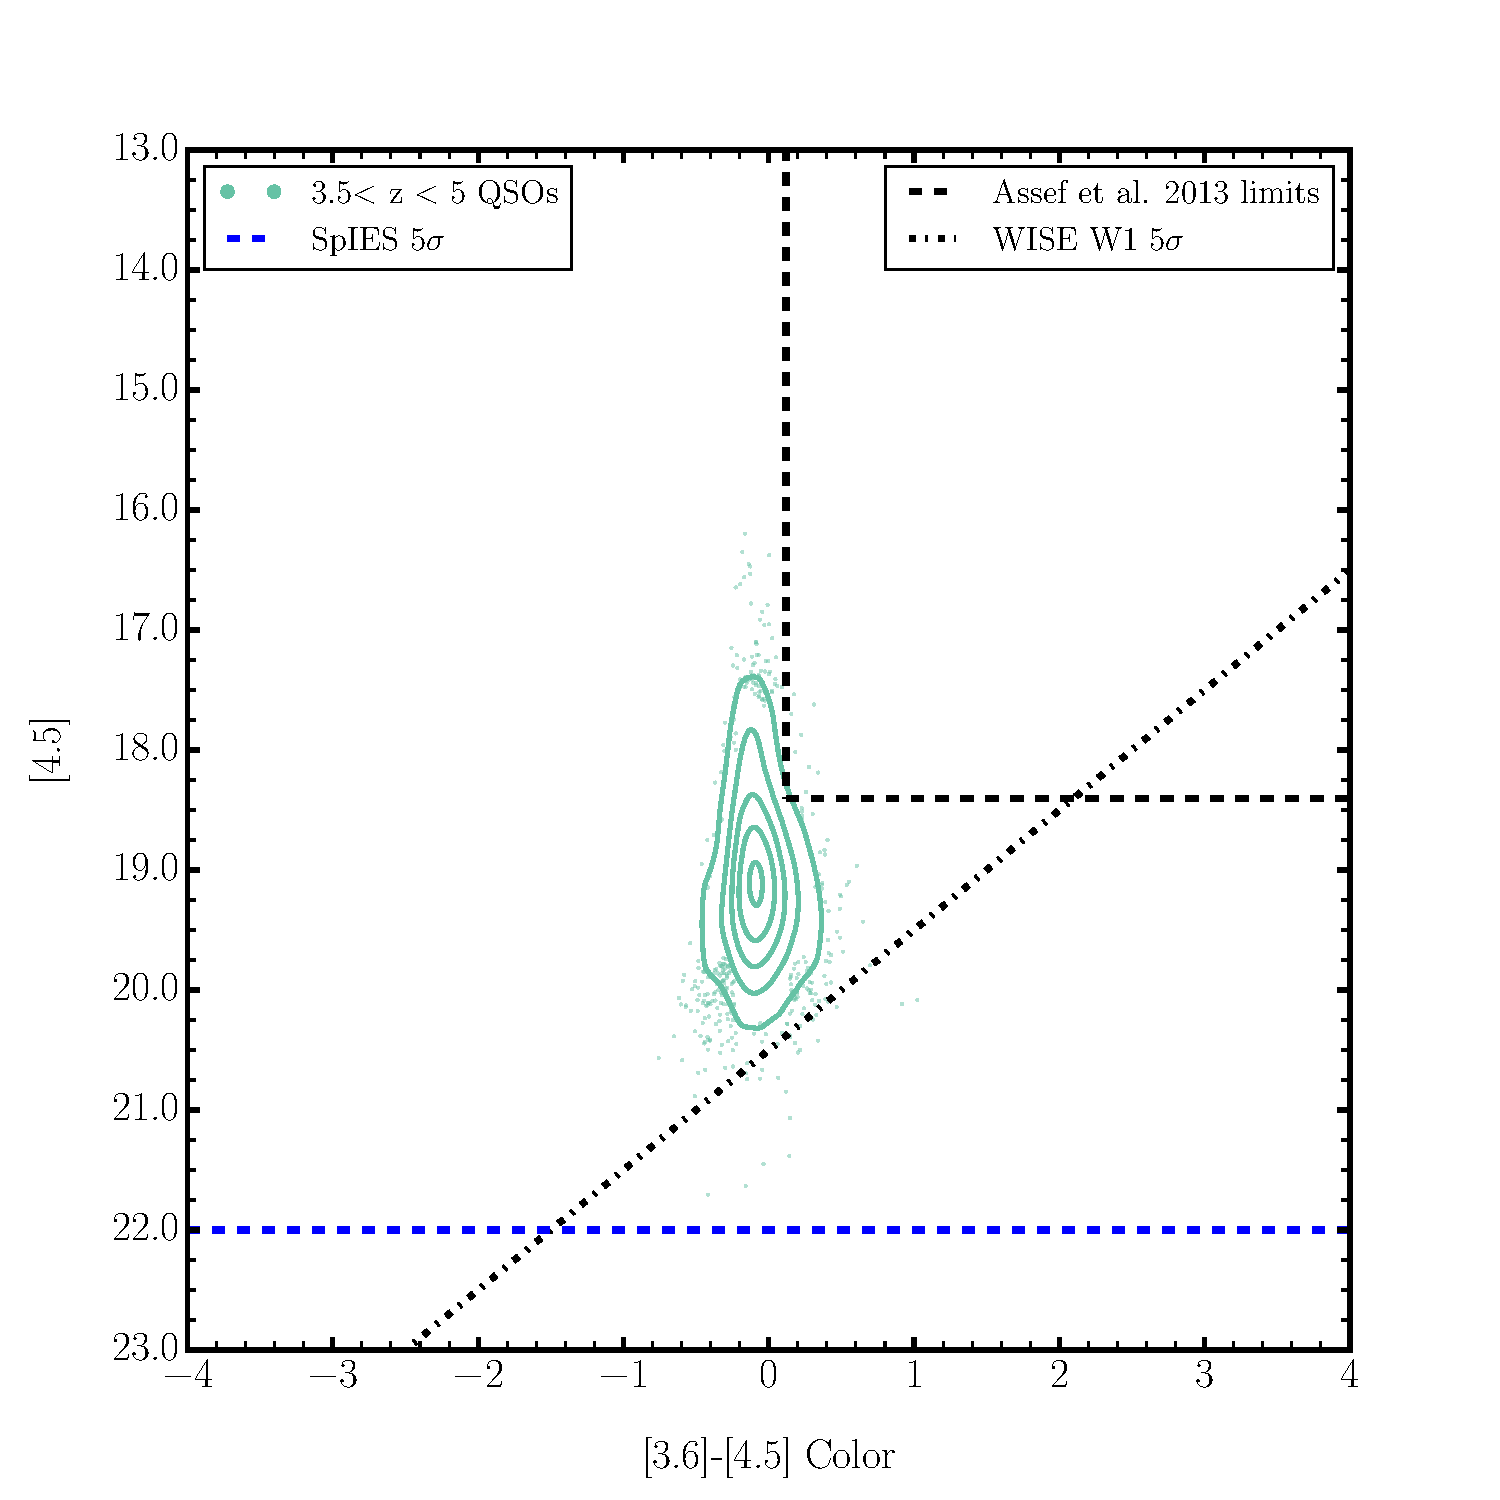
\includegraphics[width=0.45\textwidth]{Group_Plotting.pdf}
		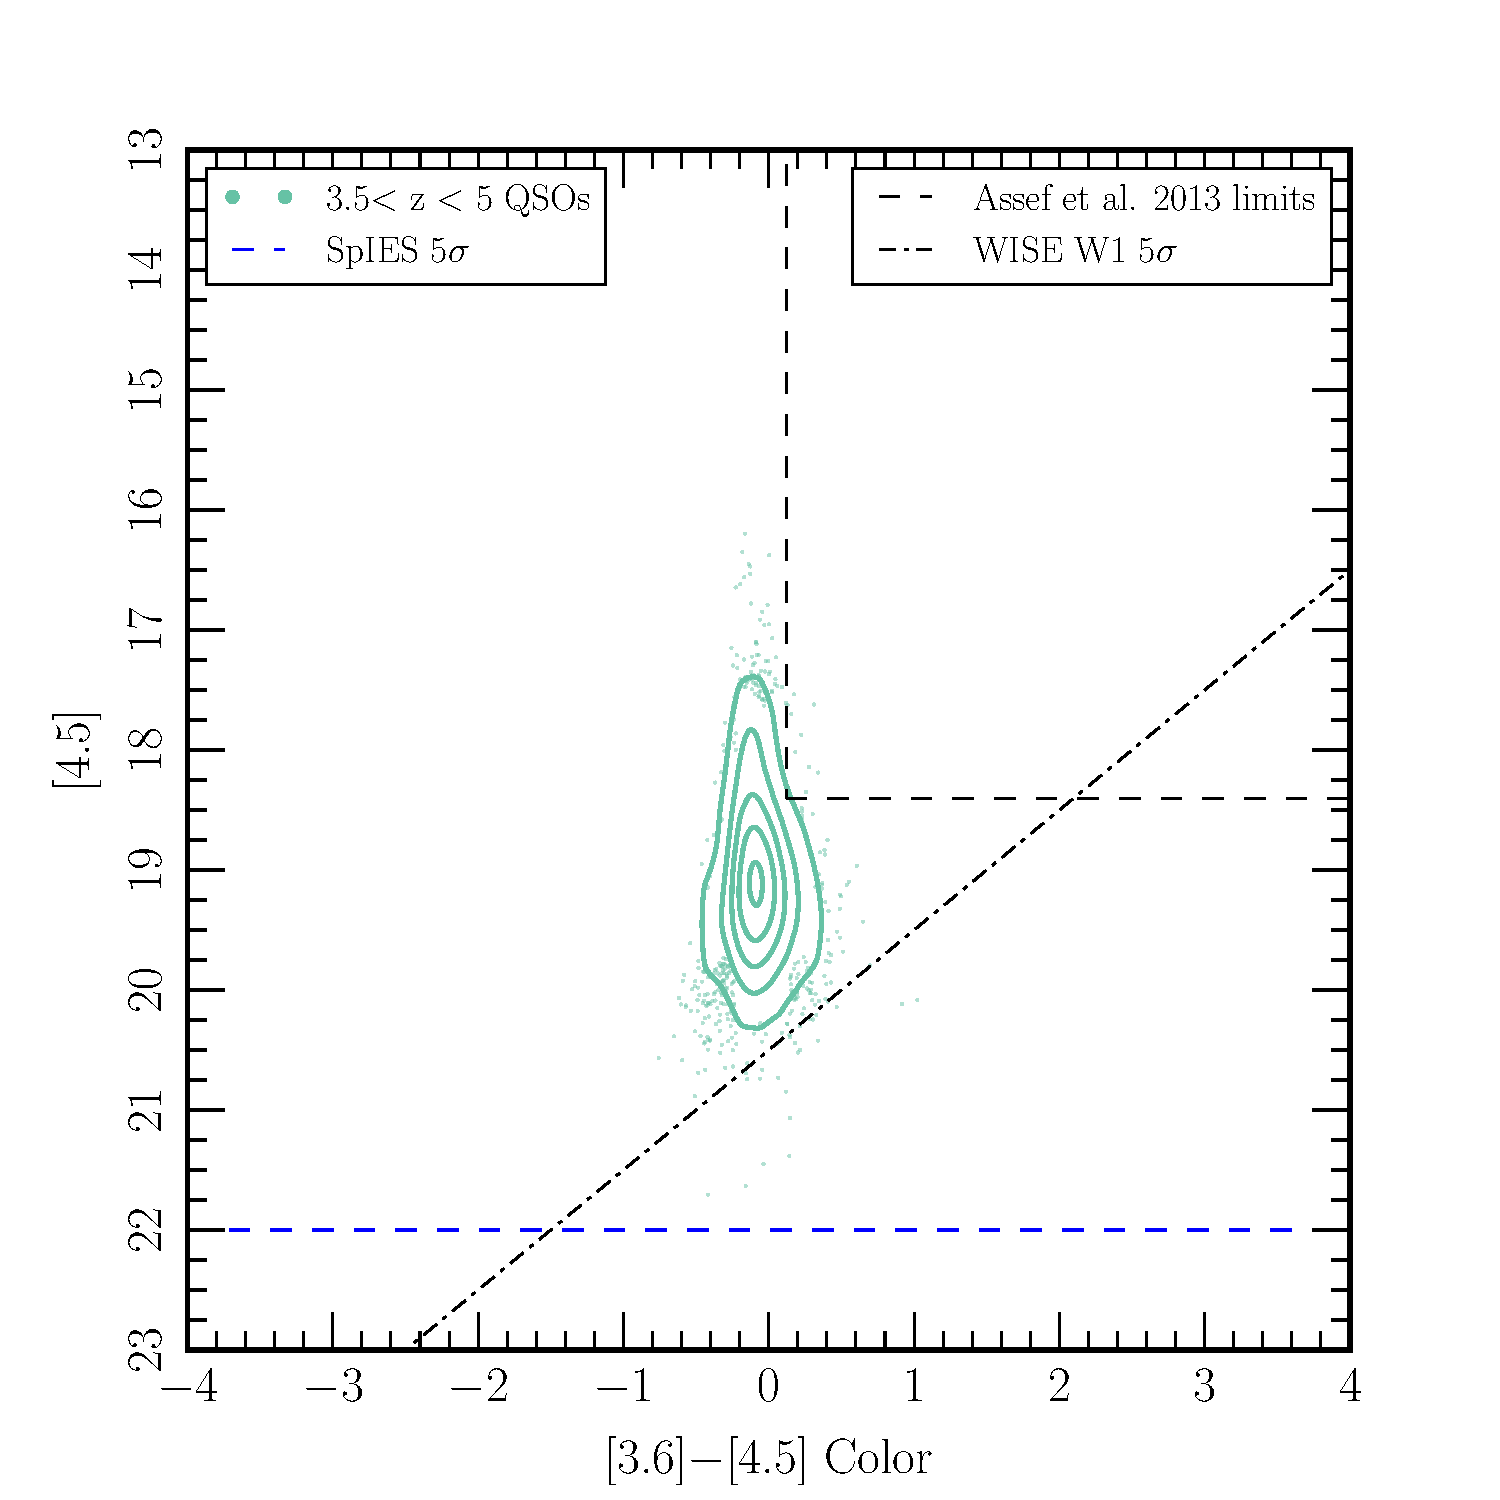
\includegraphics[width=0.45\textwidth]{Group_Plotting2.pdf}
		%\captionsetup{width=0.75\linewidth}
		\caption{\footnotesize{Changing the RC-Parameters and some of the plotting styles, you can get plots that (using the default style) look like the left hand plot to look like the right hand plot}}
		\label{spies_detections}
	\end{figure}
	
		In the plot on the right, I changed the axis width, tick mark size and width, spacing of the axis labels and numbers, and all font sizes. Additionally, I manually set the dashed line and dot-dashed line lengths (of the marks and dots) and the spaces between them.
\end{document}